\documentclass{article}
\usepackage{indentfirst}
\usepackage{graphicx}
\usepackage{listings}
\usepackage{picture}
\usepackage{graphics}
\usepackage{hyperref}
\usepackage{amsmath} % for argmax
\usepackage{bm} % used for bolding the equation

\title{Computer \& Network Security I Homework1}
\author{Chang Liu ~\\ chang\_liu@student.uml.edu}

\begin{document}
\maketitle

\section{1.5}

The captured figure is as follows:

\begin{center}
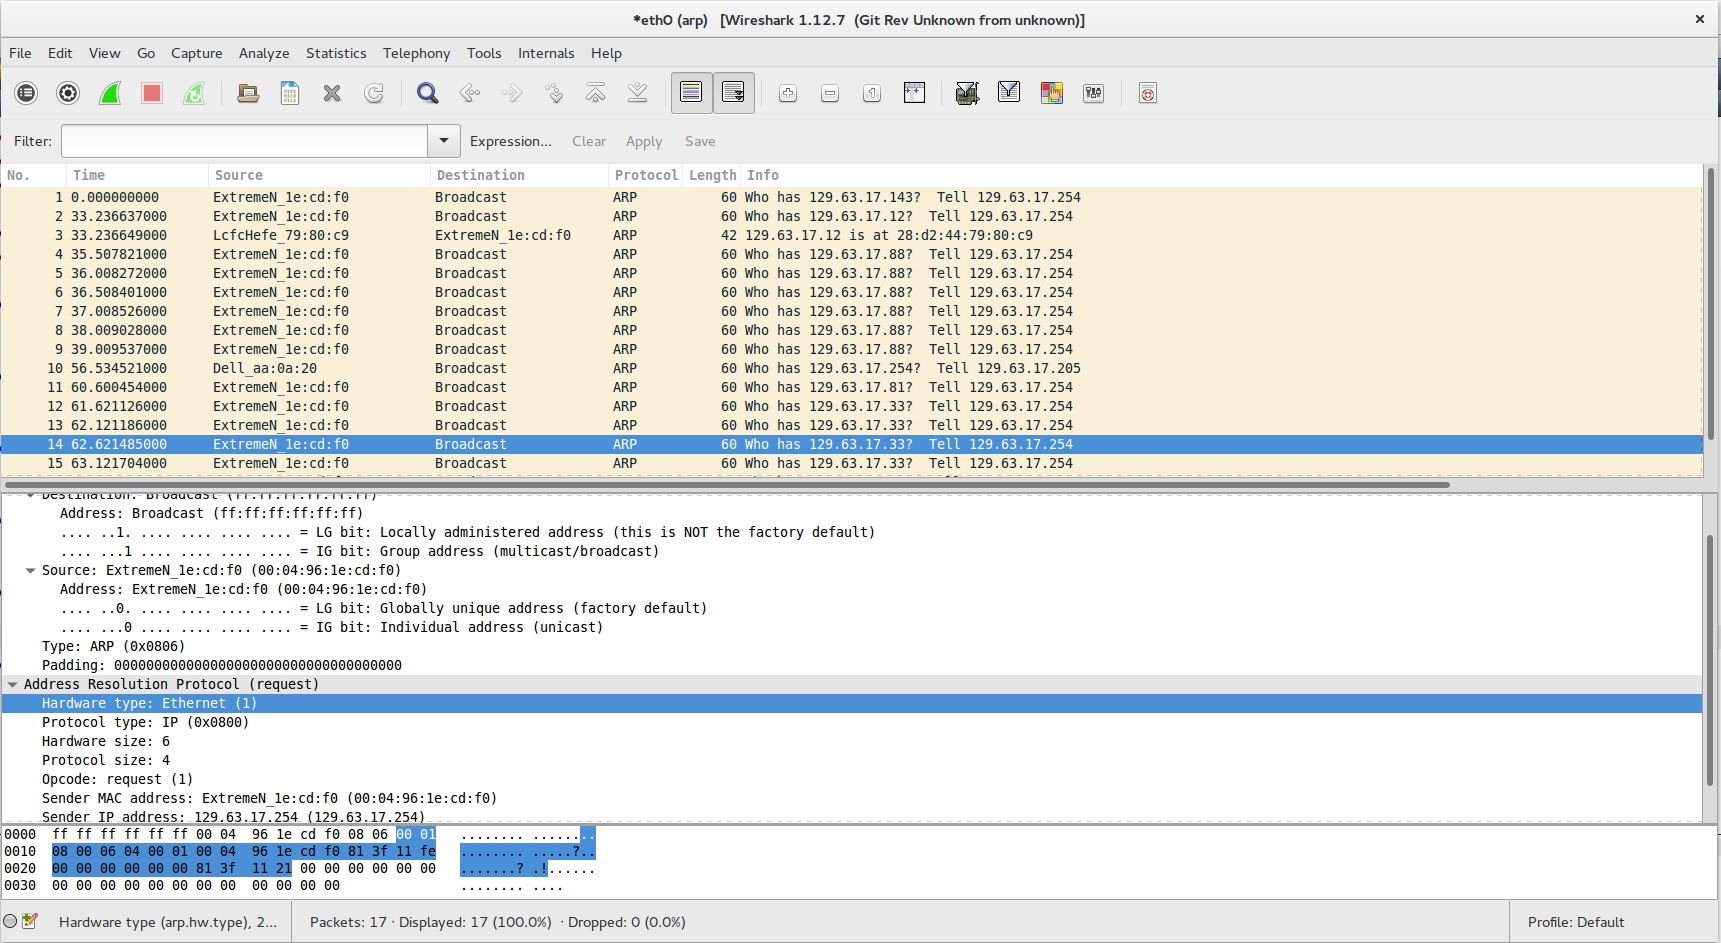
\includegraphics[scale=0.25]{hw1_fig1.png}
\end{center}

As we could see from the upper window in the figure, the ARP packages are all broadcast from the local machine with fixed MAC Address, and the length is also 60 bytes. In the `Info' field, it asked the query about `who has 129.63.17.XXX', that is destination IP address, which we
want to query for its actual MAC address.

In the middle window, there are detailed headers of the ARP packages, we can see some detailed information, for example, protocol type is `IP',
Sender MAC address is `00:04:96:1e:cd:f0', Sender IP address is `129.63.17.254', Target MAC address are all zero, because that's what we want to
query using ARP, and destination IP address is `129.63.17.33', that's the target MAC's IP address. We can also see other useful information in
the package headers.

In the lower window of the figure, that is the hexadecimal format of the ARP package, we can correspond the header information in the specific
location of this value.

As we only capture the ARP package from the steps, we can only see the ARP packages. When we use browser to visit some website, it sets up TCP/IP connections to the remote server, and finally get to know the server's IP address. But when it cannot find the target MAC address in ARP cache,
it will start the ARP query and broadcast to local network iteratively, after the target machine receives the query and return its MAC address,
it will be finally passed to the source machine and then the query is finished.

\section{1.7}

\subsection{1.7.a}
\begin{lstlisting}
char = A, count = 10, frequency  = 2.717391
char = B, count = 16, frequency  = 4.347826
char = C, count = 40, frequency  = 10.869565
char = D, count = 8, frequency  = 2.173913
char = E, count = 4, frequency  = 1.086957
char = F, count = 27, frequency  = 7.336957
char = G, count = 22, frequency  = 5.978261
char = H, count = 26, frequency  = 7.065217
char = I, count = 9, frequency  = 2.445652
char = J, count = 29, frequency  = 7.880435
char = K, count = 0, frequency  = 0.000000
char = L, count = 2, frequency  = 0.543478
char = M, count = 12, frequency  = 3.260870
char = N, count = 10, frequency  = 2.717391
char = O, count = 20, frequency  = 5.434783
char = P, count = 15, frequency  = 4.076087
char = Q, count = 9, frequency  = 2.445652
char = R, count = 3, frequency  = 0.815217
char = S, count = 23, frequency  = 6.250000
char = T, count = 57, frequency  = 15.489130
char = U, count = 0, frequency  = 0.000000
char = V, count = 8, frequency  = 2.173913
char = W, count = 4, frequency  = 1.086957
char = X, count = 2, frequency  = 0.543478
char = Y, count = 6, frequency  = 1.630435
char = Z, count = 6, frequency  = 1.630435
\end{lstlisting}

\subsection{1.7.b}

By sorting the frequence using decreasing order, we can get some corresponding relation between the two sequence,
as the following figure shows

\begin{center}
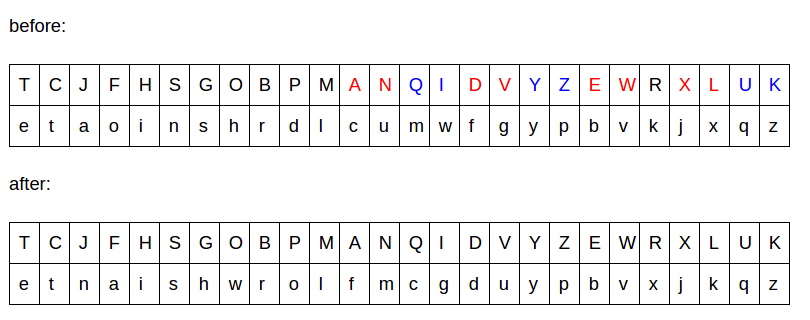
\includegraphics[scale=0.3]{fig2.png}
\end{center}

However, some order is not correct, as our sequence is not ideal and my disrupted by frequency, so we need to manually
build the relation and exclude some wrong relation, as the after shows.

After I build the relation, the new translated plain text is here as follows:
\textbf{Methods of making messages unintelligible to adversaries have been necessary.
Substitution is the simplest method that replaces a character in the plain text 
with a fixed different character in the cipher text. This methods preservers 
the letter frequency in the plain text and so one can search for the plain text
from a given cipher text by comparing the frequency of each letter against 
the know common frequency in the underlying language.}

\section{1.13}

\subsection{(a)}

Since the online game needs to communicate with the server and other player about their actions, progress, user name and account
information should be transferred as well as the game data, if these data is encrypted, then the attacker will incept these data,
analyse the field of data, and then get to know the user accounts information.

\subsection{(b)}

Yes, it will help to secure the account. Because when using the RSA token in the online game, the account information is encrypted,
the attacker can not get the plain account information from the data packets.
And this RSA token machanism is protected by the online game, they need to provide the options for better security. On their side,
a decrypted procedure is needed to verify the user's account information for management.
Still, this way is not 100\% percent safe, but it will reduce the risk significantly.

\section{1.29}

\subsection{(a)}

First, they use the technique called \textbf{Social Engineering}, they pretend to be sales person and government authority(\textit{Physical
Impersonation}), and then \textbf{Phishing} the customers, to get their email address.

Then use the \textbf{Spoofing} technique to impersonate known employees to other employees, this will allow them to send emails to victims
acting as normal employees without knowing the passwords of their disguised users.

They also used \textbf{Spam emails} with \textbf{Trojan Horse} that will get access to the internal network, they use the \textbf{Backdoors}
of the OWA system and security protocols, so that bypassing the firewall is possible and their attack is effective.


\subsection{(b)}

First, check the full email address and don't only true the display name. Some disguised emails have the host name that doesn't belong to the
authorized companies and governments, but the display is like some very formal organizations, check the full details in case we are cheated.

Second, don't click the directed link or strange url in this email. As they may contain Trojans or spyware, we can just take a look but don't
open them.

Third, watch out for some spelling errors in the emails, big companies and governments seldom send misspelled emails.

At last, watch out for asking bank account information, personal information, or other urgent or threatening information. They will use these
information to do harmful things and steal your money. Keep an on the body and content of these emails, if necessary, make a phone call that is
verified by the officials, rather than the phone number or address in the emails. Also keep an eye on the attached and executed programs in the
emails.

\section{1.37}

The new security policy should forbid the placing of computers behind the firewall, and place ALL the computers under the protect of the firewall.

Furthermore, new monitoring mechanism should be built to watch the behaviour of network and other security benchmark. Once there is an abnormal
activity, it should be easy to locate the area of problem, and them minimize the search boarder of suspicious computers. In this way, it would
be easy to localize the compromised computer.

And other isolation network should be built so that if there is some victims, the system will shut down the communication between these machines
and other connected machine. In this way, the transmission of virus can be slowed down and the affected machine can be minimized.

At last, make sure every computer has install the anti-virus software, even some old computers, this will largely reduce the risk of infecting other computers. Scan and check the computer periodically to avoid infections.




\end{document}